\begin{frame}{ProtBERT: A Protein Language Model}
\setbeamercovered{transparent}
    \begin{columns}
        % Left column for text
        \column{0.6\textwidth}
        \textbf{Overview}
        \vspace{0.5em}
        \begin{itemize}
            \item<1> \textbf{ProtBERT} is a pre-trained language model specifically designed for proteins.
            \item<2> It uses a \textbf{transformer architecture} similar to BERT, but adapted for protein sequences.
        \end{itemize}
        
        % Right column for images
        \column{0.4\textwidth}
        \begin{center}
            \only<1>{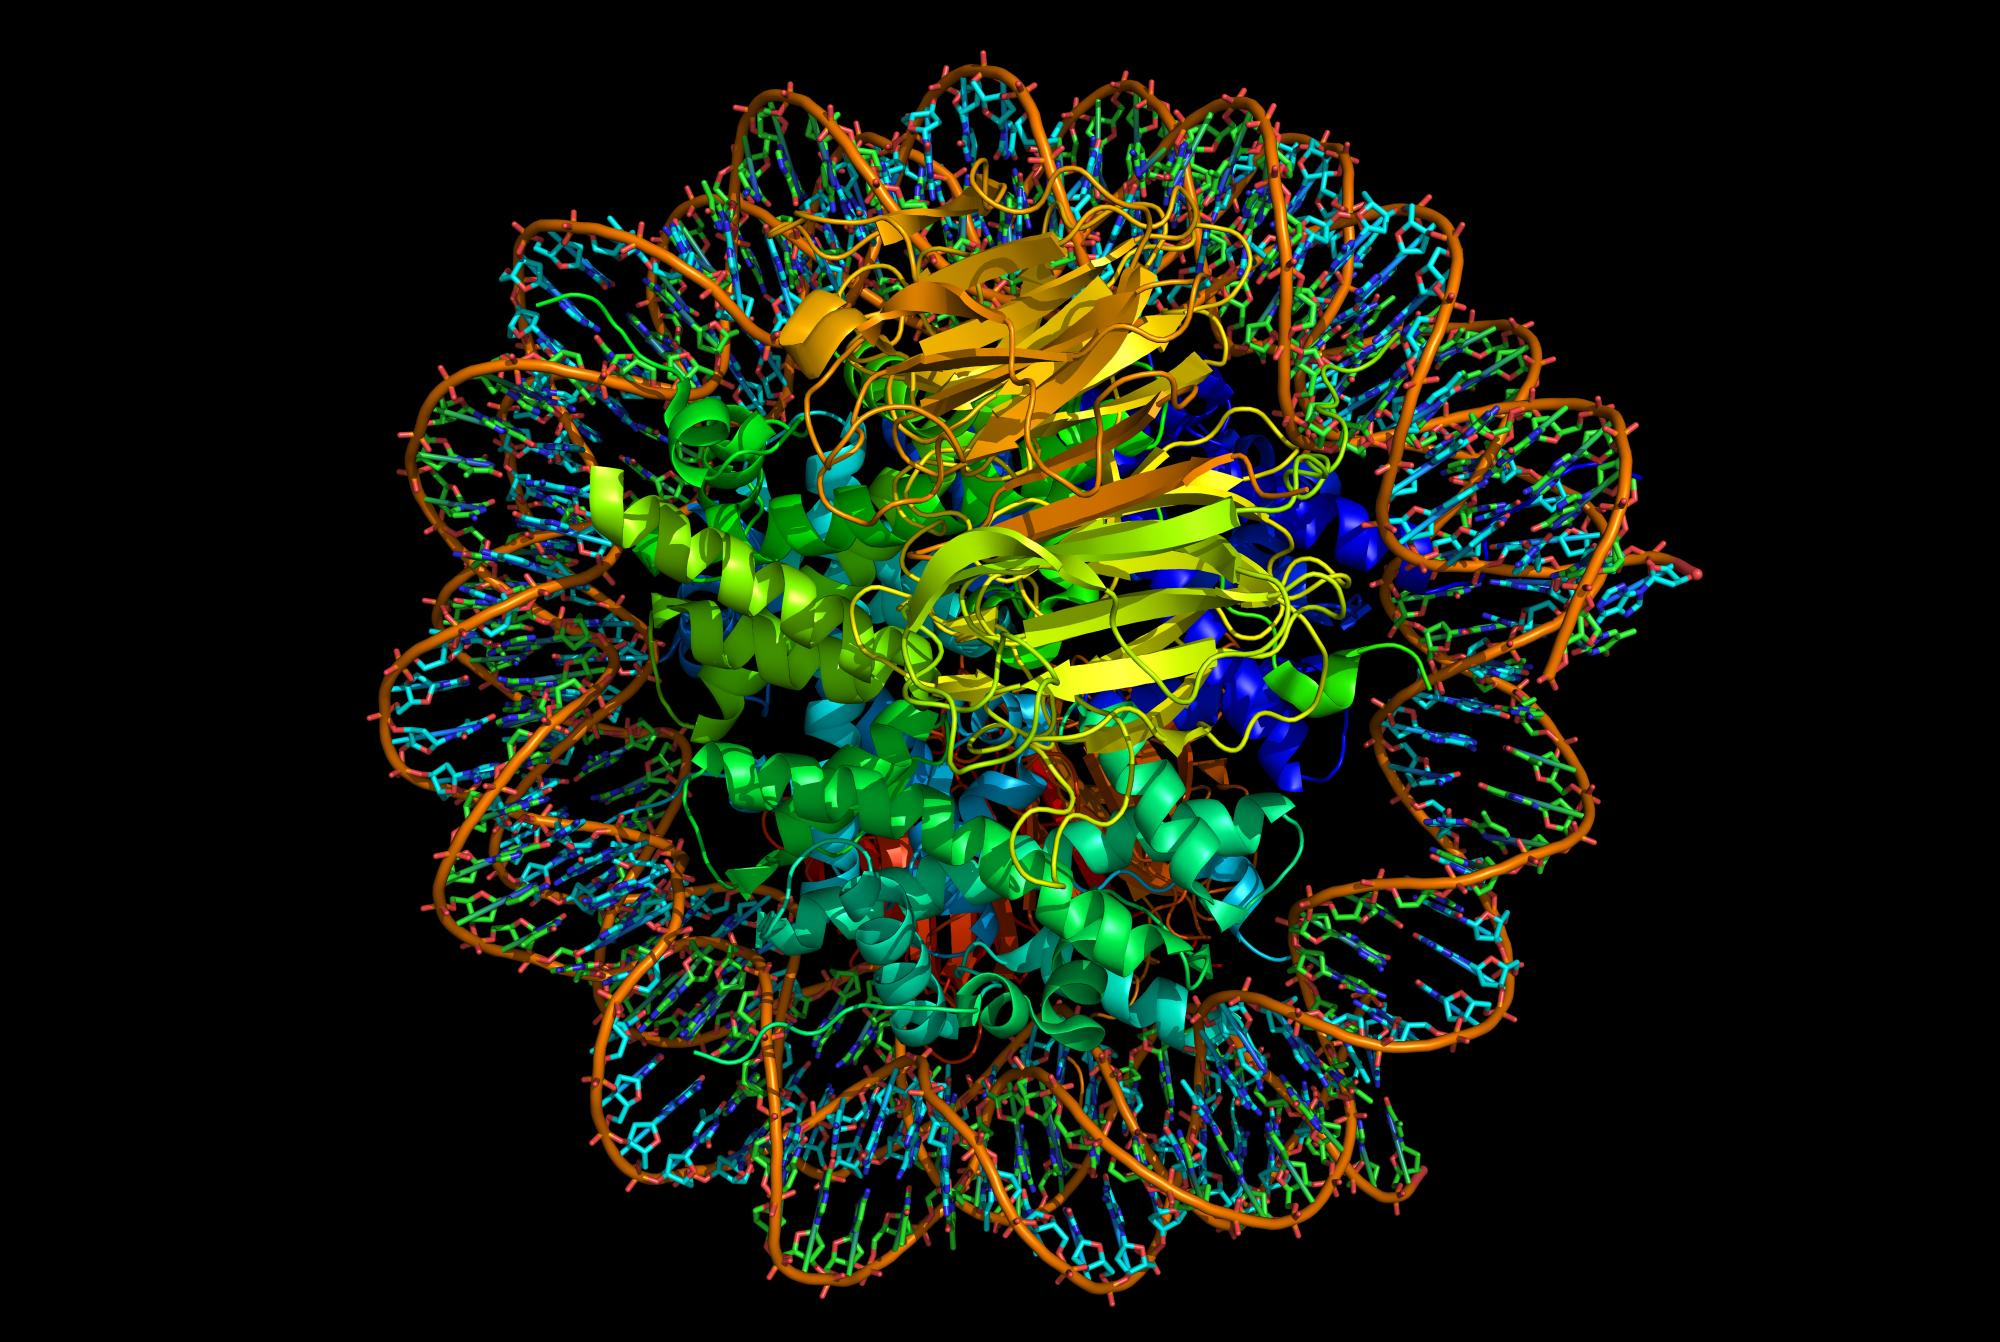
\includegraphics[width=\textwidth]{images/nucleosome.jpeg} \\ }
            \vspace{1em}
            \only<2>{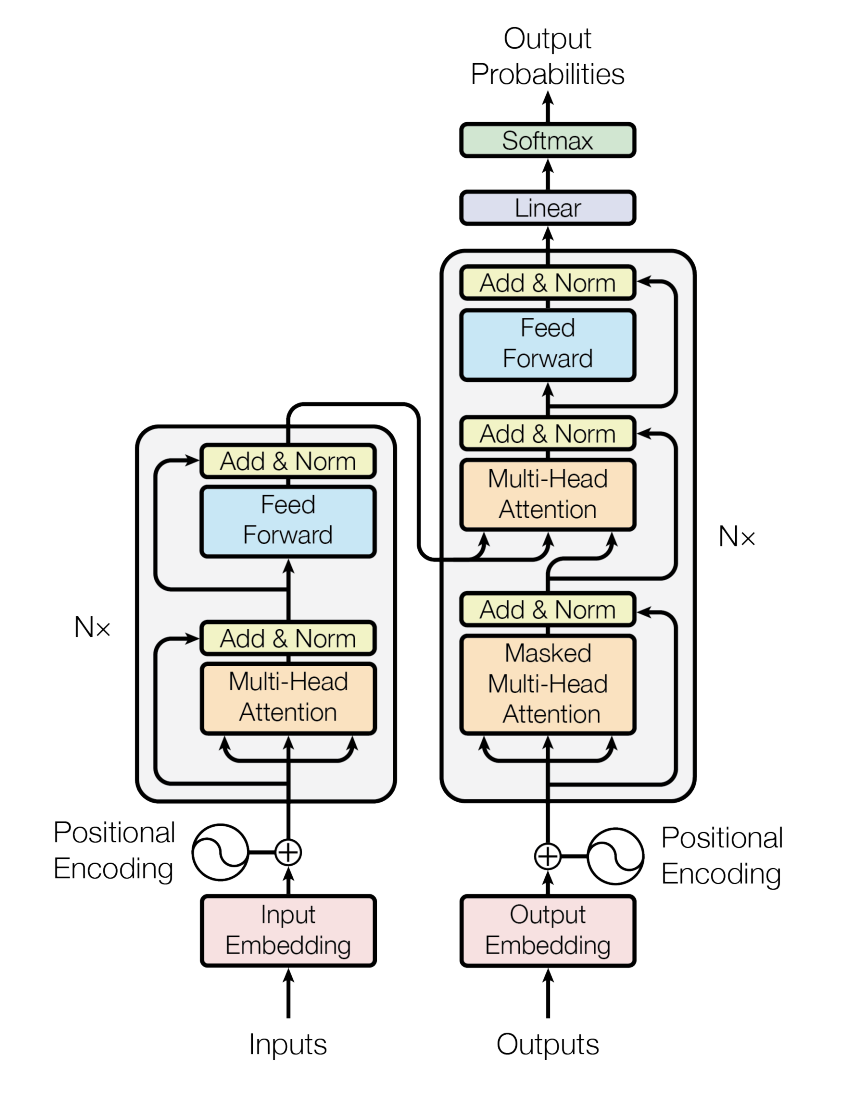
\includegraphics[width=\textwidth]{images/transformers.PNG} }
        \end{center}
    \end{columns}
\end{frame}


\begin{frame}
    \frametitle{ProtBERT: Key Features}
    \begin{columns}
        % Left Column: Tasks
        \column{0.45\textwidth}

        \begin{center}
            \begin{tikzpicture}[
                node distance=0.3cm and 1.2cm,
                align=center,
                rounded corners,
                every node/.style={},
                input/.style={draw, fill=lightblue2!50, text width=4cm, minimum height=1.5cm},
                arrow/.style={-Stealth, thick},
                scale=0.8
            ]

            % Tasks
            \visible<1>{\node[input, opacity=1] (structure) {Tokenization:
Breaks protein
sequences into
k-mers (short
overlapping
substrings).};}
            \visible<2->{\node[input, opacity=.2] (structure) {Tokenization};}
            
            \visible<2>{\node[input, below=0.9cm of structure, opacity=1] (interactions) {Pre-training:
            Utilizes unsupervised learning with masked language modeling.};}
            \visible<1, 3->{\node[input, below=0.9cm of structure, opacity=.2] (interactions) {Pre-training};}
            
            \visible<3>{\node[input, below=0.9cm of interactions, opacity=1] (mutation) {Transfer Learning: Can be fine-tuned for tasks such as protein function prediction and protein structure prediction};}
            \visible<1-2>{\node[input, below=0.9cm of interactions, opacity=.2] (mutation) {Transfer Learning};}

        \end{tikzpicture}
        \end{center}

        % Right Column: Models
        \column{0.55\textwidth}
        \begin{center}
            \begin{tikzpicture}[
                node distance=0.3cm and 1,
                align=center,
                rounded corners,
                every node/.style={},
                input/.style={draw, fill=greyblue!40, text width=4cm, minimum height=.8cm},
                output/.style={draw,fill=white!10, text width=5cm, minimum height=.8cm},
                arrow/.style={-Stealth, thick},
                scale=0.8
            ]
            \only<1>{
                % \node {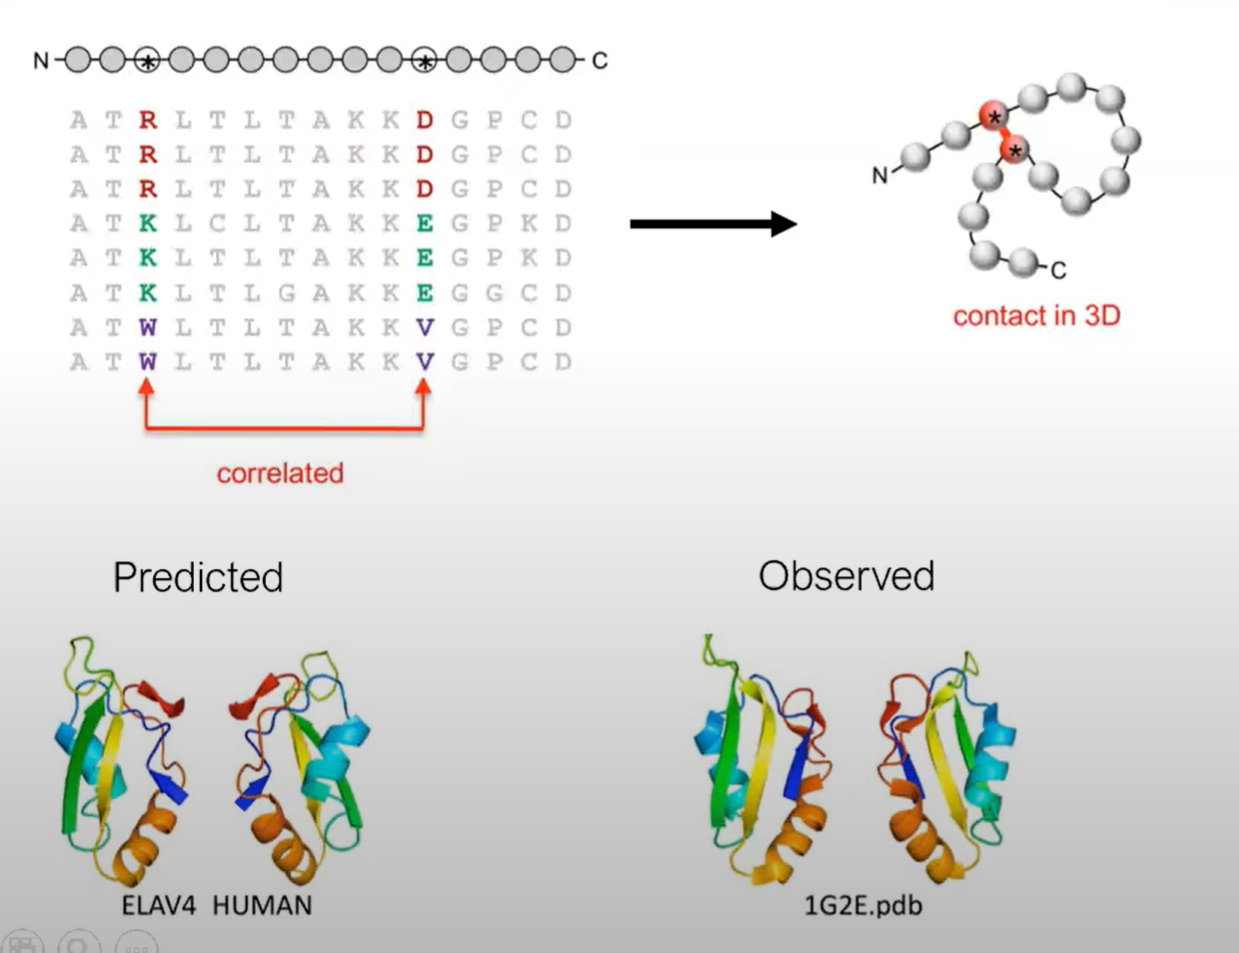
\includegraphics[width=\textwidth]{images/stdetr.png}};
                \node[](alpic) at (0,3.5) {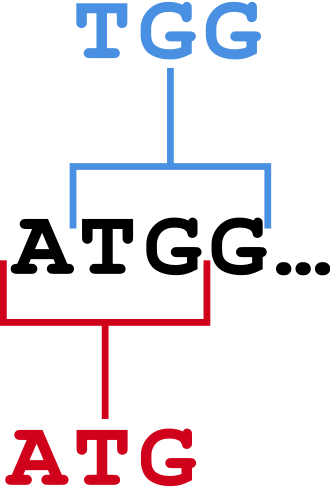
\includegraphics[width=3cm, keepaspectratio]{images/K-mer_diagram.svg.png}};
            }
             \only<2>{
                \node[](pipic) at (0,3.5) {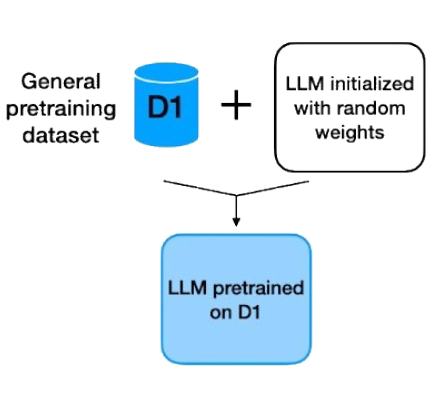
\includegraphics[width=5cm, keepaspectratio]{images/pretraining.PNG}};
            }
            \only<3>{
               \node[] (mutpic) at (0,3.5) {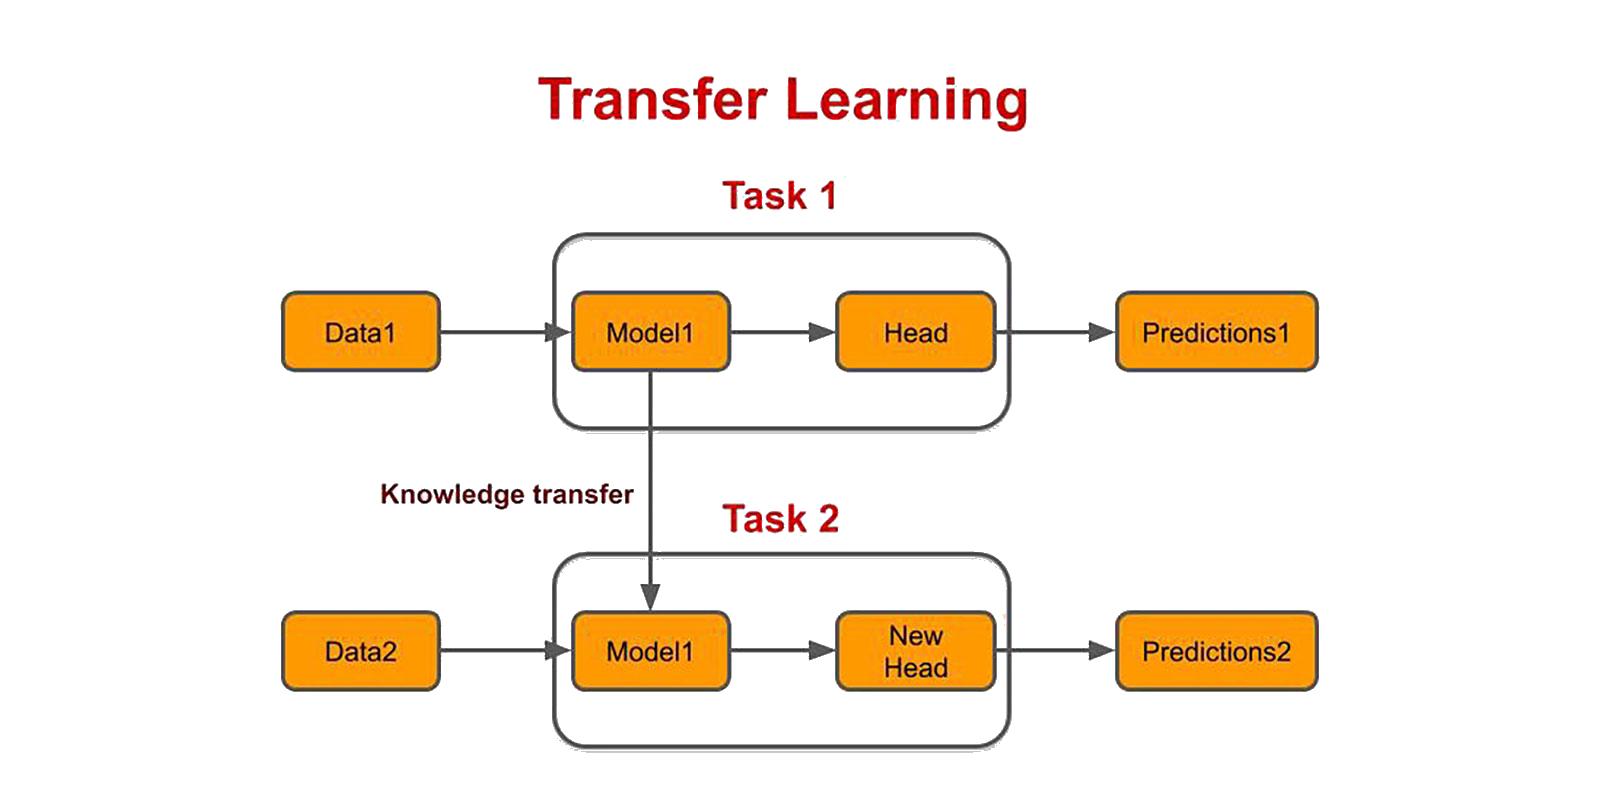
\includegraphics[width=7cm, keepaspectratio]{images/transfer_learning.PNG}};
            }
            

        \end{tikzpicture}
        \end{center}
    \end{columns}
\end{frame}



